\documentclass[journal]{IEEEtran}
\usepackage[a5paper, margin=10mm]{geometry}
%\usepackage{lmodern} % Ensure lmodern is loaded for pdflatex
\usepackage{tfrupee} % Include tfrupee package


\setlength{\headheight}{1cm} % Set the height of the header box
\setlength{\headsep}{0mm}     % Set the distance between the header box and the top of the text


%\usepackage[a5paper, top=10mm, bottom=10mm, left=10mm, right=10mm]{geometry}

%
\setlength{\intextsep}{10pt} % Space between text and floats

\makeindex


\usepackage{cite}
\usepackage{amsmath,amssymb,amsfonts,amsthm}
\usepackage{algorithmic}
\usepackage{graphicx}
\usepackage{textcomp}
\usepackage{xcolor}
\usepackage{txfonts}
\usepackage{listings}
\usepackage{enumitem}
\usepackage{mathtools}
\usepackage{gensymb}
\usepackage{comment}
\usepackage[breaklinks=true]{hyperref}
\usepackage{tkz-euclide} 
\usepackage{listings}
\usepackage{multicol}
\usepackage{xparse}
\usepackage{gvv}
%\def\inputGnumericTable{}                                 
\usepackage[latin1]{inputenc}                                
\usepackage{color}                                            
\usepackage{array}                                            
\usepackage{longtable}                                       
\usepackage{calc}                                             
\usepackage{multirow}                                         
\usepackage{hhline}                                           
\usepackage{ifthen}                                               
\usepackage{lscape}
\usepackage{tabularx}
\usepackage{array}
\usepackage{float}
\usepackage{ar}
\usepackage[version=4]{mhchem}


\newtheorem{theorem}{Theorem}[section]
\newtheorem{problem}{Problem}
\newtheorem{proposition}{Proposition}[section]
\newtheorem{lemma}{Lemma}[section]
\newtheorem{corollary}[theorem]{Corollary}
\newtheorem{example}{Example}[section]
\newtheorem{definition}[problem]{Definition}
\newcommand{\BEQA}{\begin{eqnarray}}
\newcommand{\EEQA}{\end{eqnarray}}

\theoremstyle{remark}


\begin{document}
\bibliographystyle{IEEEtran}
\onecolumn

\title{9.4.40}
\author{INDHIRESH S- EE25BTECH11027}
\maketitle


\renewcommand{\thefigure}{\theenumi}
\renewcommand{\thetable}{\theenumi}

\textbf{Question}.A train travels 360 km at a uniform speed. If the speed had been 5 km/hr more, it would have taken 1 hour less for the same journey. Find the speed of the train.\\
\textbf{Solution}:\\
Let us solve the given equation theoretically and then verify the solution computationally. \\
Let the uniform speed of the train be s km/hr.\\
Let the time taken for the journey be t hours.\\
From 1st journey:
\begin{align}
   360=s\times t
\end{align}


\begin{align}
  t=\frac{360}{s}
\end{align}
For the second scenario:
\begin{align}
 360=(s+5)(t-1)
\end{align}
Now substitute Eq.2 in Eq.3
\begin{align}
  360=(s+5)(\frac{360}{s}-1)
\end{align}

\begin{align}
  s^2+5s-1800=0
\end{align}
Let
\begin{align}
    u= s^2+5s-1800
\end{align}
This can be expressed as:
\begin{align}
  \Vec{x^T}\Vec{V}\Vec{x} + 2\Vec{u^T}\Vec{x} + f = 0
\end{align}
Where,
\begin{align}
    \Vec{x}=\myvec{s\\u}\;\; ,\Vec{V}=\myvec{1&0\\0&0}\;\;,\Vec{u}=\myvec{2.5\\-0.5}\;\;and\;\;f=-1800
\end{align}
Now finding the point of intersection of parabola with s-axis:
\begin{align}
    \Vec{x}=\Vec{h}+k\Vec{m}
\end{align}
\begin{align}
    \Vec{h}=\myvec{0\\0}\;\;and\;\;\Vec{m}=\myvec{1\\0}
\end{align}
\begin{align}
    \Vec{x}=k\myvec{1\\0}
\end{align}
Now substitute Eq.11 in Eq.7

\begin{align}
k^2\myvec{1\\0}^T\myvec{1&0\\0&0}\myvec{1\\0}+2\myvec{2.5\\-0.5}^Tk\myvec{1\\0}-1800=0
\end{align}

\begin{align}
  k^2+5k-1800=0
\end{align}

\begin{align}
   k=\frac{-5\pm \sqrt{25-4(-1800)}}{4}
\end{align}

\begin{align}
    k=40\;\;and \;\;k=-45
\end{align}
Speed cannot be negative. So,
\begin{align}
    k=40
\end{align}
Substitute in Eq.11
\begin{align}
   s=40\;km/hr
\end{align}



From the figure it is clearly verified that the theoretical solution matches with the computational solution.\\
\begin{figure}[h]
    \centering
    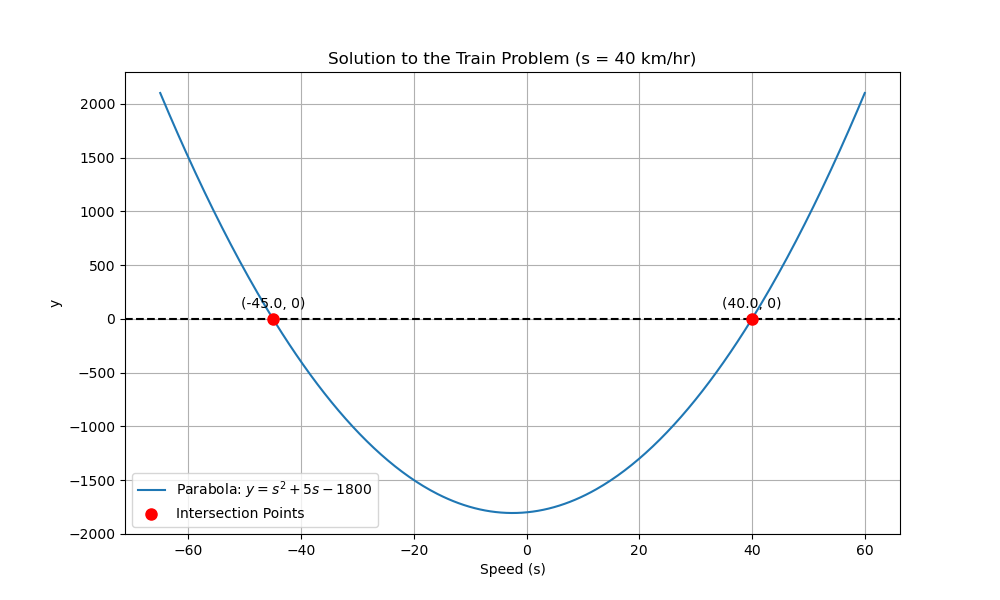
\includegraphics[height=0.5\textheight, keepaspectratio]{figs/figure1.png}
    \label{figure_1}
\end{figure}

\end{document}